\documentclass[10pt]{beamer}

\usepackage[utf8]{inputenc} 
\usepackage[T1]{fontenc}
\usepackage{lmodern}
\usepackage{graphicx}
\usepackage[english]{babel}
\usepackage{listings}
 %\usepackage{bbm}
\usepackage{color}
\usetheme{Warsaw}
\usepackage{lmodern}
\newtheorem{prop}{Proposition}
\usepackage{epsfig}
\setlength\abovecaptionskip{0.03ex}

 
\begin{document}
 
\title{\textbf{Backward Stochastic Differential Equation}}
\author{ Majdi Rabia}
\maketitle

\AtBeginSection[]
{
  \begin{frame}
  \frametitle{Sommaire}
  \tableofcontents[currentsection,currentsubsection, hideothersubsections]
  \end{frame} 
}


\section{Introduction}

\begin{frame}
	\frametitle{Motivation}
	
	\begin{block}{Example of a Stock Graph}
	
	
	\centering
	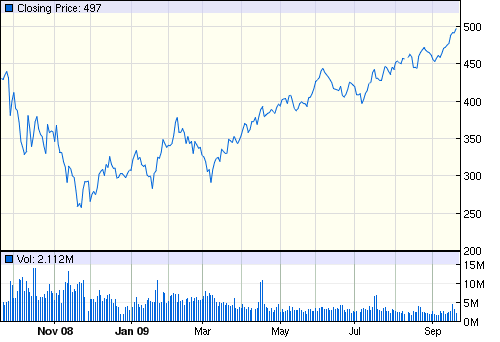
\includegraphics[scale=0.5]{motivation.png}
\end{block}
	
	
\end{frame}



 \begin{frame}
 \frametitle{American Option}


\begin{block}{Objective}
	\begin{itemize}
		\item Let $t \in [0,T]$
		\item Payoff at time $T$: 
		\[V_T = (S_T - K)^+\]
		\item We can exercise at any stopping time between $[0, T]$
		\item Hence, we would like, with $g : x\rightarrow (x - K)^+$, to maximize $\mathbb{E}[g(S_t)]$ from today to maturity. 
		\[V_0 = \sup_{t \in \tau}\mathbb{E}[g(S_t)]\]
		with $\tau$ the set of stopping times
	\end{itemize}
\end{block}

 \end{frame}
 
 
 
 \section{BSDE}
 
 \begin{frame} 
 	
 	
 	\frametitle{Forward Diffusion}
 	
 	
 	
 	\begin{block}{Model}
 		
 			\begin{eqnarray}
 			dX_t = \mu(t,X_t)dt + \sigma (t, X_t) dB_t\notag
 			\end{eqnarray}
 			
 	\end{block}
 	
 	\pause
 	
 	
 	\centering
 	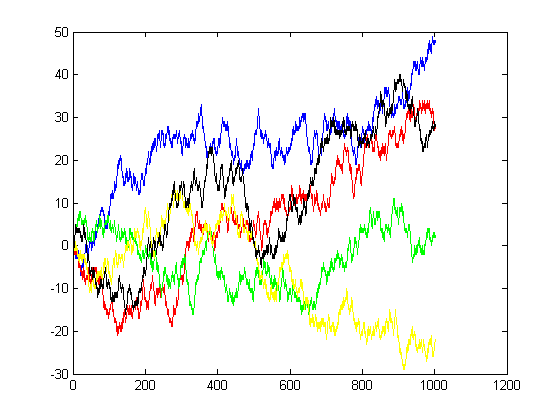
\includegraphics[scale=0.4]{random_walk.png}
 	
 \end{frame}
 
 
 
 \begin{frame} 
 	
 	
 	\frametitle{Backward}
 		
 		
 		
 		\begin{block}{Model}
 
 				\begin{eqnarray}
 				dX_t = \mu(t,X_t)dt + \sigma (t, X_t) dB_t\notag\\
 				-dY_t = f(t,X_t, Y_t, Z_t)dt - Z_tdB_t \notag\\
 				Y_T=\xi (X_T) \notag
 				\end{eqnarray}
 				
 				\pause
 				
 				Where :
 				
 				\begin{itemize}
 					\item f is called the driver 
 					\item $Z_t$ is a stochastic process related to $u(t,X_t) = Y_t$ by : 
 					\[Z_t = \sigma(t, X_t) Du_x (t, X_t)\]
 					\item $\xi$ is a measurable function
 				\end{itemize}
 	
 		\end{block}
 		
 \end{frame}
 
\begin{frame} 


	\frametitle{Backward}
	
	
	
	\begin{block}{Example : European Option}
	
			The driver for a European Option with a Geometric Brownian motion model for $X_t$ and using risk neutral measure : 
			
			\begin{eqnarray}
			f(t,X_t, Y_t, Z_t) = - r Y_t
			\end{eqnarray}
		
	\end{block}
	
\end{frame}

\begin{frame}
	
	
	\begin{block}{Proof}
		\begin{eqnarray}
		dY_t & =& \underbrace{\phi_t}_{\text{amount invested in stock}} \frac{dX_t}{X_t} + (Y_t - \phi_t)rdt \notag\\
		dY_t &=&r\phi dt + \sigma dB_t + (Y_t - \phi_t)rdt \notag\\
		dY_t &=& rY_tdt + \sigma \phi dB_t\notag \\
		- dY_t &=& - rY_tdt - Z_t dB_t 
		\end{eqnarray}
		\end{block}

\end{frame}


\section{Solving BSDE's}

\begin{frame}
	\frametitle{Discretization}
	
	
	\begin{displaymath}
	Z_{t_i} = \frac{1}{\Delta t_i}\mathbb{E}[Y_{t_{i + 1}} \Delta B_{t_i}  | \mathcal{F}_{t_i}]
	\end{displaymath}
	
	\begin{displaymath}
	Y_{t_i} = \mathbb{E}[Y_{t_{i + 1}} | \mathcal{F}_{t_i}] +  f(t_i,S_{t_i}, Y_{t_{i + 1}}, Z_{t_i})\Delta t_i
	\end{displaymath}
	
\end{frame}


\section{Conditional Expectation : numerical solutions}

   \begin{frame}
   	\frametitle{Mesh Method : Glasserman}
   	\centering
   	 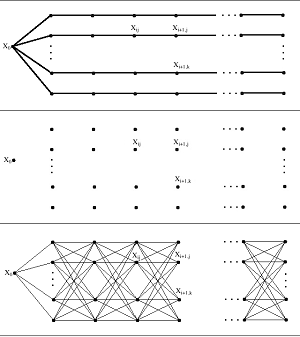
\includegraphics[scale = 0.6]{mesh_figure.png} 
   	 

   	
   \end{frame}
  
  
   \begin{frame}
   	\frametitle{Mesh Method : Glasserman}
   	
   	\begin{block}{Propositon}
   		\[\mathbb{E}[Y_{t_{i + 1}}^j | (X_{t_{i + 1}})] = \sum_{j=1}^{N} W_{i, k}^jY_{t_{i + 1}}^j\]
   		
   		the weights being given by the properties of the diffusion 
   		
   	\end{block}
   	
   \end{frame}
    \begin{frame}
    	\frametitle{Tree Regression : Random Forest}
    	\centering
    	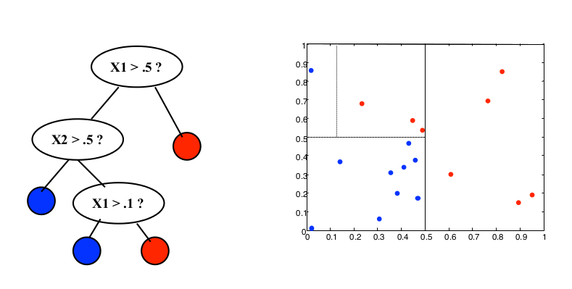
\includegraphics[scale = 0.6]{rf.png} 
    \end{frame}

	 \begin{frame}
	 	\frametitle{Tree Regression : Gradient Boosting}
	 	\centering
	 	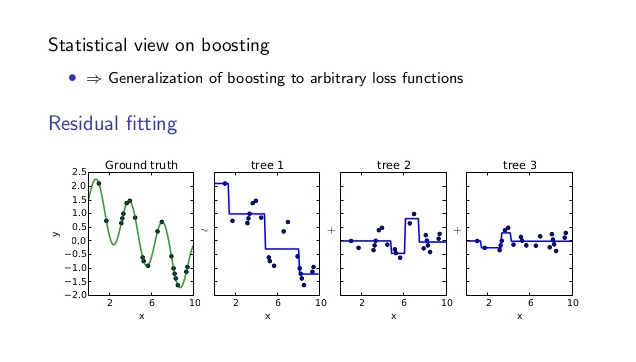
\includegraphics[scale = 0.6]{grad_boost.png} 
	 \end{frame}
	 
	 \begin{frame}
	 	\frametitle{Using BSDE properties}
	 	
	 	$Z_{t_i} = \frac{1}{\Delta t_i}\mathbb{E}[Y_{t_{i + 1}} \Delta B_{t_i}  | \mathcal{F}_{t_i}]$includes a very noisy process to approximate. 
	 	\pause
	 	
	 	\vspace{1cm} 
	 	We make use of :  $Z_t = \sigma(t, X_t) Du_x (t, X_t)$  where $u(t, X_t) = Y_t$
	 	
	 	\pause
	 
	 	
	 	\begin{itemize}
	 		\item 1 : $Z_{t_i} = \frac{1}{\Delta t_i}\mathbb{E}[Y_{t_{i + 1}} \Delta B_{t_i}  | \mathcal{F}_{t_i}]$ with one of previous methods 
	 		\item 2 : $Y_{t_i} = \mathbb{E}[Y_{t_{i + 1}} | \mathcal{F}_{t_i}] +  f(t_i,S_{t_i}, Y_{t_{i + 1}}, Z_{t_i})\Delta t_i$
	 			\end{itemize}
	 	We use then a Picard Iteration (considering this as a Markovian case): 
	 	\begin{itemize}
	 		\item 3 : We approximate $Y_{t_i} = \hat{h}(t_i, X_{t_i})$
	 		\item 4  : $Z_{t_i} = \sigma(t_i, X_{t_i}) \nabla\hat{h}(t_i, X_{t_i})$
	 	\end{itemize}
	 	
	 	This gives a more stable $Z_t$ process at time t. 
	 	
	 \end{frame}
	 
\section{Simulations}

\begin{frame}
	\frametitle{Bid-ask Spread Option}
	
	\begin{block}{driver in this case}
		\[
		\left\{
		\begin{aligned}
		f(t,Y_t,Z_t) & =  -Z_t\theta  - rY + (R-r)(Y-\frac{Z_t}{\sigma})^-\\
		\theta &= \frac{\mu - r}{\sigma}\\
		\xi(X_T) & = (X_T - K_1) - 2(X_T - K_2)
		\end{aligned}
		\right.
		\]	
	
	\end{block}
	\centering
	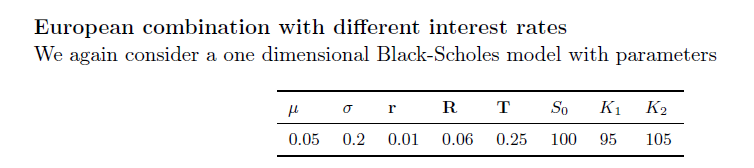
\includegraphics[scale = 0.5]{bid_ask.png} 
	
\end{frame}

\begin{frame}
	\frametitle{Gobet use of Hypercubes regression}
	

	\centering
	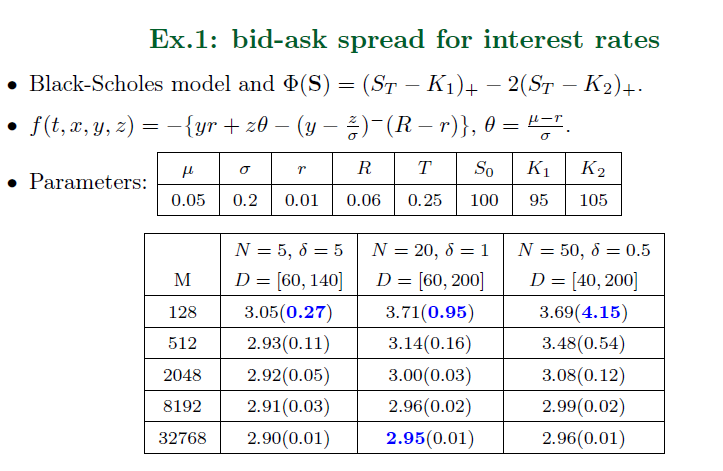
\includegraphics[scale = 0.4]{gobet_results.png} 
	
\end{frame}

\begin{frame}
	\frametitle{Our Results}
	
	
	\centering
	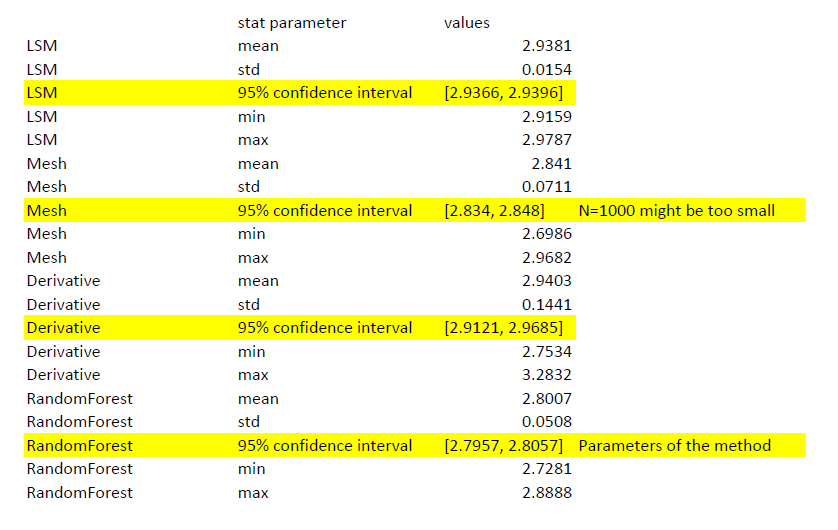
\includegraphics[scale = 0.4]{our_results.png} 
	
\end{frame}

\section{American Option}

\begin{frame}
	\frametitle{RBSDE and American Option}
	\begin{block}{Model}
		\begin{eqnarray}
		dX_t = \mu(t,X_t)dt + \sigma (t, X_t) dB_t\notag\\
		-dY_t = f(t,X_t, Y_t, Z_t)dt - Z_tdB_t +dL_t\notag\\
		Y_T=\xi (X_T) \notag \\
		\int_{0}^{T}(Y_t - \xi(X_t))dL_t = 0\notag
		\end{eqnarray}
	\end{block}
	
	$L_t$ controls $Y$ to stay above the barrier $\xi$
\end{frame}

\section{What's next now}

\begin{frame}
	\begin{itemize}
		\item High dimension with Random Forest currently looks good, need to optimize the parameters and use multithreading to get competitive simulations and publish. 
		
		\pause
		\item Adapt the Process to 2-BSDE, which requires more computation !
		\pause
		\item Create a mapping non-linear PDE $\rightarrow$ to 2-BSDE
		\pause
		\item Clean the code, comment and put on Github for open source.  
	\end{itemize}
\end{frame}


\section{Acknowledgements}
\begin{frame}
	

Thanks to : 
\newline
\textbf{Alexandre Thiery }(NUS, Department of Applied Probability and Statistics) 
\newline
 \textbf{Zhou Chao} (NUS, Department of Mathematics) 
 \newline
 for supporting me throughout this research. 

\end{frame}
 
\end{document}